\section{Infix Proofs}
Since we do not provide any new contribution to the infix proofs under soft fork conditions, we provide the algorithms for the full infix proofs construction as well as a high level description of the construction. These are needed in order to keep up with the novelties described later in the velvet infix proofs section. For a more detailed presentation of this construction, the reader should refer to~\cite{nipopows}. Most of this section's content is borrowed from~\cite{nipopows}.

By requesting a suffix proof a client can synchronize to the latest valid chain or learn about information that can be extracted by the last $k$ block of the chain. Nevertheless, suffix proofs act as the stepping stone for the construction of another useful class of proofs, which answer to more general predicates that can depend on multiple blocks buried deep within the blockchain.

More specifically, an \emph{infix proof} allows proving any predicate $Q(\chain)$ that depends on a number of blocks that may appear anywhere within the chain (excpet for the last $k$ block for stability reasons). These blocks consitute a subset $\chain'$ of blocks, the \emph{witness}, which may not necesserily form a stand-alone subchain. This allows proving useful queries such as, whether a transaction is confirmed.

The following definition formally states the notion of an \emph{infix-sensitive} predicate.

\begin{definition}[Infix Sensitivity]
    A chain predicate $Q_d,k$ is infix sensitiveif it can be written in the form 
    \begin{equation*}
        Q_{d,k}(\chain) =
        \begin{cases}
             \text{true, if } \exists \chain' \subseteq \chain[:-k] : \lvert \chain' \rvert \leq d \wedge D(\chain')\\
            \text{false, otherwise}
        \end{cases}
    \end{equation*}
    Where D is an arbitrary computable predicate.
\end{definition}

The construction of infix proofs is given in Algorithms~\ref{alg:infix_prover_soft_fork},~\ref{alg:followDown_soft_fork}. The infix prover accepts as parameters the full blockchain $\chain$ and the subset $\chain'$ which contains the blocks of interest fro answering a specific predicate in question. the prover calls the suffix prover algorithm to produce a proof $(\pi, \chi)$ for $\chain$. Then, the infix prover adds some auxiliary blocks to the poof prefix $\pi$, ensuring that these auxiliary blocks form a chain with the rest of the blocks in $\pi$. Such auxiliary blocks are collected as follows. For every block of interest $B$ of the subset $\chain'$, the immediate previous ($E'$) and immediate next ($E$) superblocks in $\pi$ are found. Then, a chain $R$ which connects $E$ back to $B'$ is found by the algorithm \textsf{followDown}. $B'$ contains a pointer to $E'$ in its interlink completing the chain. Observe that $B'$ necessarily includes a pointer to $E'$ because of the choice of $E'$.

\begin{algorithm}[h!]
	\caption{\label{alg:infix_prover_soft_fork}The Infix Prover for the superblock NIPoPoW protocol~\cite{nipopows}}
	\begin{algorithmic}[1]
      \Function{\sf ProveInfix$_{m,k}$}{$\chain, \chain', \text{depth}$}
          \Let{(\pi, \chi)}{\textsf{Prove}_(m,k)(\chain)}
          \For{$B' \in \chain'$}
              \For{$E \in \pi$}
                  \If{$\textsf{depth}(E) \geq \textsf{depth}(B')$}
                      \Let{R}{\textsf{followDown}(E, B', \textsf{depth})}
                      \Let{aux}{aux \cup R}
                      \textbf{break}
                  \EndIf
                  \Let{E'}{E}
              \EndFor
          \EndFor
          \State\Return $(aux \cup \pi, \chi)$
      \EndFunction
	\end{algorithmic}
\end{algorithm}

The \textsf{followDown} algorithm proceeds as follows. Starting from block $hi = E$, it tries to follow a pointer to as far as possible without surpassing the block of interest $B'$. Any pointer that surpasses $B'$ is aborted and a pointer of lower is tried, which causes a smaller step within the skiplist. If a pointer was folllowed without surpassing $B'$, the operation continues from the new pointed block, until eventually $B'$ is reached. An example execution is illustrated in Figure~\ref{fig:infix_soft_fork}.

\begin{figure}[h!]
	\begin{center}
		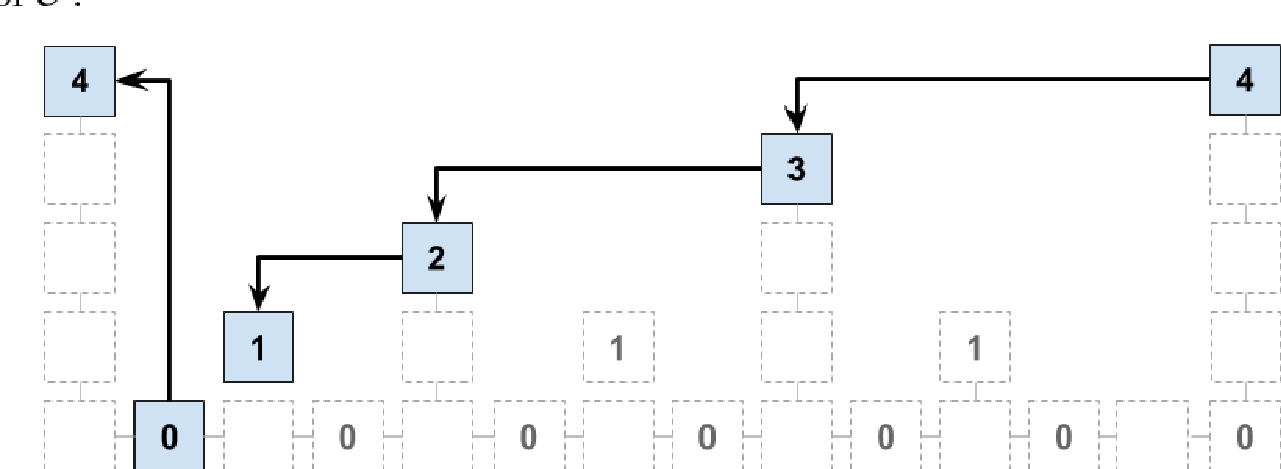
\includegraphics[width=0.73\textwidth]{figures/infix.pdf}
	\end{center}
	\caption{An infix proof descend. Only blue blocks are included in the proof.Blue blocks of level 4 are part of $\pi$, while the blue blocks of level 1 to 3 are produced by the \textsf{followDown} to get to the block of level 0, which is part of $\chain'$.} 
	\label{fig:infix_soft_fork}
\end{figure}

The verification algorithm is given in Algorithm~\ref{alg:infix_verifier_soft_fork}. The algorithm calls the suffix verifier. It maintains a block-DAG collecting blocks from all proofs received, i.e. all proofs in $\mathcal{P}$. 
This DAG is maintained in the \textsf{blockById} hashmap. Using it, \textsf{ancestors} uses simple graph search to extract the set of ancestor blocks of a block of interest. In the final predicate evaluation the set of ancestors of the best chain tip's is passed to the predicate. The ancestors are included to avoid an adversary who presents an honest chain but skips the block of interest from the auxiliary blocks in the infix proof.
%Why construct a whole DAG than just examine every chain that has equivalent PoW in the corresponding suffix proof.

\begin{algorithm}[h!]
	\caption{\label{alg:followDown_soft_fork}The $\textsf{followDown}$ function which produces the necessary blocks to connect a superblock \textit{hi} to a preceding regular block \textit{lo}~\cite{nipopows}}
	\begin{algorithmic}[1]
      \Function{\sf ProveInfix$_{m,k}$}{$\chain, \chain', \text{depth}$}
        \Let{B}{\textit{hi}} 
        \Let{\textit{aux}}{\text{[ ]}} 
        \Let{\mu}{\textit{level}(hi)}
        \While{$B \neq \textit{lo}$}
            \Let{B'}{\textsf{blockById}[\text{B.interlink}[\mu]]}
            \If{$\textsf{depth}[B'] < \textsf{depth}[lo]$}
                \Let{\mu}{\mu - 1}
            \Else
                \Let{aux}{ aux \cup B}
                \Let{B}{B'}
            \EndIf
        \EndWhile
        \State\Return$aux$
      \EndFunction
	\end{algorithmic}
\end{algorithm}

\begin{algorithm}[h!]
	\caption{\label{alg:infix_verifier_soft_fork}The $\textsf{verify}$ algorithm for the superblock NIPoPoW infix protocol~\cite{nipopows}}
	\begin{algorithmic}[1]
      \Function{\sf ancestors}{$B, \textsf{blockById}$}
        \If{$B = Gen$}
            \State\Return$\{ B \}$
        \EndIf
        \Let{\chain}{\emptyset}
        \For{$B' \in B.\textsf{interlink}$}
            \Let{\chain}{\chain \cup \textsf{ancestors}(B')}
        \EndFor
        \State\Return$\chain \cup B$
      \EndFunction
      \vspace{2mm}
      \Function{$\textsf{verify-infix}^D_{l,m,k}$}{$\mathcal{P}$}
        \Let{\textsf{blockById}}{\emptyset}
        \For{$(\pi, \chi) \in \mathcal{P}$}
            \For{$B \in \pi$}
                \Let{\textsf{blockById}[B.id]}{B}
            \EndFor
        \EndFor
        \Let{\tilde{\pi}}{\text{best } \pi \in \mathcal{P} \text{ according to suffix verifier}}
        \State\Return$D(\textsf{ancestors}(\tilde{\pi}[-1], \textsf{blockById}))$
      \EndFunction
	\end{algorithmic}
\end{algorithm}
